\documentclass[a4paper]{article}

\usepackage[a4paper]{geometry}

\usepackage{setspace}
\singlespacing

\usepackage{graphicx}
\graphicspath{{/home/adzlan/Documents/proRep1920_1/figure/}}
\usepackage[sumlimits,]{amsmath}

\usepackage[]{SIunits}

\usepackage[
  backend=biber,
  style=authoryear-icomp
]{biblatex}

\addbibresource{literature.bib}

\begin{document}

%The macros for freestream velocities
\newcommand{\uon}{\unit{0.1}{\metre\per\second}}
\newcommand{\utw}{\unit{0.2}{\metre\per\second}}
\newcommand{\uth}{\unit{0.3}{\metre\per\second}}
\newcommand{\ufo}{\unit{0.4}{\metre\per\second}}
\newcommand{\ufi}{\unit{0.5}{\metre\per\second}}
\newcommand{\usi}{\unit{0.6}{\metre\per\second}}
\newcommand{\use}{\unit{0.7}{\metre\per\second}}
\newcommand{\uei}{\unit{0.8}{\metre\per\second}}
\newcommand{\uni}{\unit{0.9}{\metre\per\second}}
\newcommand{\ute}{\unit{1.0}{\metre\per\second}}
\newcommand{\uel}{\unit{1.1}{\metre\per\second}}
\newcommand{\utv}{\unit{1.2}{\metre\per\second}}
\newcommand{\utt}{\unit{1.3}{\metre\per\second}}

%The macros for plate tilt angle
\newcommand{\ptlt}{$\theta_{\text{plate}}$}
\newcommand{\rze}{\unit{0}{\radian}}
\newcommand{\ron}{\unit{\pi/8}{\radian}}
\newcommand{\rtw}{\unit{\pi/4}{\radian}}
\newcommand{\rth}{\unit{3\pi/8}{\radian}}
\newcommand{\rfo}{\unit{\pi/2}{\radian}}

%The macros for commonly used symbols
\newcommand{\ypl}{$y^{+}$} %yPlus
\newcommand{\ured}{$U^{*}$} %reduced velocity
\newcommand{\yrms}{$y^{*}_{\text{RMS}}$} %root-mean-square of the normalised cylinder displacement

\newcommand{\uron}{$2.3$}
\newcommand{\urtw}{$4.5$}
\newcommand{\urth}{$6.8$}
\newcommand{\urfo}{$9.1$}
\newcommand{\urfi}{$11.4$}
\newcommand{\ursi}{$13.6$}
\newcommand{\urse}{$15.9$}
\newcommand{\urei}{$18.2$}
\newcommand{\urni}{$20.5$}
\newcommand{\urte}{$22.7$}
\newcommand{\urel}{$25.0$}
\newcommand{\urtv}{$27.3$}
\newcommand{\urtt}{$29.5$}

\newcommand{\es}{$=$}

\section{Title of thesis}
Micro-watt energy harvesting by exploiting the flow around a circular cylinder-strip plate cruciform

\section{Project outline} \label{outline}
This work seeks to exploit the flow-induced vibration (FIV) due to vortex shedding around a circular cylinder--strip plate cruciform to generate power. The circular cylinder is elastically mounted, and the periodic shedding of the vortices create the alternate lift that drives the vibration of the cylinder.

In a pure cruciform configuration between the cylinder and plate, i.e. both aretilted \rfo{} to each other, a vibration response is elicited from the elastically mounted cylinder that exceeds the maximum vibration amplitude of an isolated cylinder, under similar flow conditions. This is desirable from an energy harvesting perspective since a higher vibration amplitude translates into higher harnessable energy from the fluid stream.

What sets off the high amplitude vibration in the cruciform setup? What is the limit for improvement for the amplitude response? How can we generalise the cruciform setup as a method for flow and vibration control? These are the questions that we seek to answer in this study.

\section{Data collection} \label{collection}
We studied the questions raised in \S\ref{outline} through the use of numerical methods to solve the continuity and Navier-Stokes equations around the problem geometery previously defined. We opted for the open source C++ library OpenFOAM due to its portability in case file management (the whole case are just text files placed in a directory tree that obeys a simple convention) and extensibility in terms of the solution of the governing equations, dynamic mesh handling and workflow customisation and automation (which is possible simply by using shell scripts or by using Python, through PyFOAM).

We collect field data such as velocity, pressure and vorticity from the numerical results to visually grasp key points in the temporal evolution of the fluid-structure interaction between the cruciform and the stream. This lays the qualitative base to our description and understanding of the flow field. We also collect one-dimensional time series data of the lift coefficient and also mean turbulent velocity fluctuations at certain locations downstream the cylinder for quantitive analysis of the vibration response.

To generalise the cruciform setup of circular cylinder-strip plate as a method for vibration response control, we varied the tilt angle of the plate, relative to the axis of the cylinder, in from \rze{} to \rfo{} in increments of \ron{}. This allows us to gauge how sensitive the vortical structures driving the vibration are with respect to structural symmetry.

\section{Data analysis} \label{analysis}

\subsection{Methods of analysis}

The one-dimensional time series data, which is oscillatory in nature, are analysed for their root-mean-square amplitude values and dominant frequency content to reveal amplitude and frequency response of the system with respect to the reduced velocity \ured{}. The dominant frequency of the system, is generally determined via fast Fourier transform (FFT) for the cylinder displacement time series (or ``signal'' for short). The root-mean-square (RMS) amplitude for the lift signal however, is computed after the signal is decomposed using ensemble empirical mode decomposition (EEMD) \parencite{Huang1998,Wu2008}, and its prevalent frequency, after computing the Hilbert spectrogram of the decomposed lift signal. We discuss why in the following paragraph.

In our past leg of study which focussed on the \rfo{} case, we observed that the lift signal behaves less sinusoidal with the advent of streamwise vortex and streamwise vortex-induced vibration (SVIV). In fact, following EEMD, we identified two components of that decomposition (also known as intrinsic mode functions or IMF) with the highest RMS amplitude, and computed their Hilbert spectrograms. What results is the discovery that these two IMFs--two with the largest RMS amplitudes--oscillate at a mean frequency close to the shedding frequency of Karman vortex (or simply the Karman frequency) while the other, oscillates close to the natural frequency of the system. Our choice of using EEMD to compute the Hilbert spectrogram allows us to gain a better understanding not only of the principal constituents of lift signal frequency, but also its temporal evolution and more generally, the degree of dispersion of the instantaneous frequencies from the mean. 

\subsection{Generalising the pure cruciform configuration}

Figure \ref{fig:ampresp} summarises the amplitude responses of the cylinder with varying \ured{} and \ptlt{}. We chose to study the effect of \ptlt{} variation in addition to \ured{} because variation of \ptlt{} is one of the most straightforward ways to generalise the \rfo{} case which is a pure cruciform configuration. The \rfo{} case is now just one of the infinite cruciform possibilities in which the plate is tilted from \rze{} to \rfo{}. This not only is the first attempt to grasp the sensitivity of the system to cruciform symmetry, but is also potentially a method to control the contribution of the streamwise and Karman vortices towards the total lift amplitude.

At \ptlt{}\es{}\rze{}, the amplitude response shows a tremendously different trend compared to the reference case of \ptlt{}\es{}\rfo{}: the root-mean-square value of the normalised cylinder displacement \yrms{} starts its growth from a very low \ured{} of \urfo{}, monotonically increases up to \ured{}\es{}\urei{}, before saturating close to \yrms{}$\approx 0.8$ at that \ured{}. We hypothesize that this form of amplitude response is  the result of the strengthening of streamwise vorticity across the spanwise direction of the cylinder. Where previously the streamwise vorticity is amplified into a sustainable flow structure only in the vicinity of the strip plate, the \rze{} plate destabilises the streamwise vorticity along the length of the cylinder, thus bringing into realisation multiple streamwise vortices simultaneously. This brings the transition to streamwise vortex-dominant regime down to \ured{}\es{}\urfo{} and imposes a larger lift on the cylinder compared to the \rfo{} case. We remind the reader that although not at \rfo{}, the plate at \rze{} is definitely a symmetrical configuration. This symmetry is broken once we rotate the plate by \ron{}, which we discuss next.

\begin{figure}[h]
  \centering
  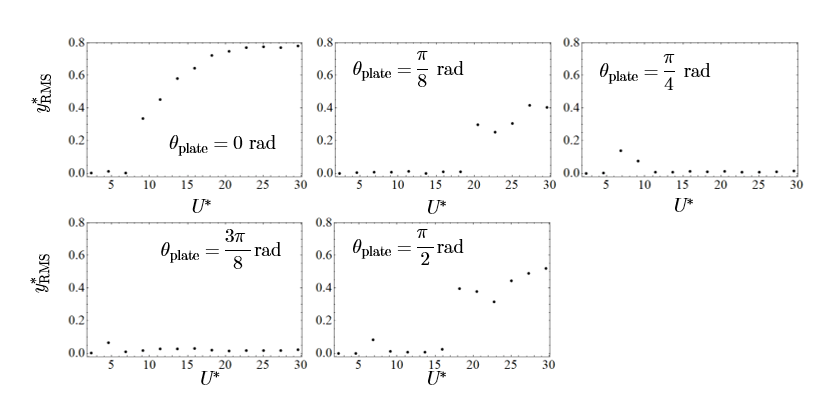
\includegraphics[width=1.0\textwidth]{amplitudeResponse.png}
  \caption{Amplitude response for the \rze{} case.}
  \label{fig:ampresp}
\end{figure}

At \ptlt{}\es{}\ron{}, the symmetry of the cylinder-plate configuration is broken. This pushes the start of the vibration regime up to a higher \ured{}\es{}\urni{}. This is an indication that the shear layer instabilities along the cylinder must be stronger compared to when \ptlt{}\es{}\rze{}, for the now asymmetrical strip plate to have an effect on the amplification and sustenance of the streamwise vorticity, which is responsible for the high-amplitude response from the cylinder. We also observe that even at the same \ured{}, the root-mean-square amplitude of vibration is smaller for the case of \ron{} as can be seen from the \yrms{} values \ured{} \es{} \urni{} through \urtt{}. $U^{*}=20.5$.

\newpage

\begin{figure}[h]
  \centering
  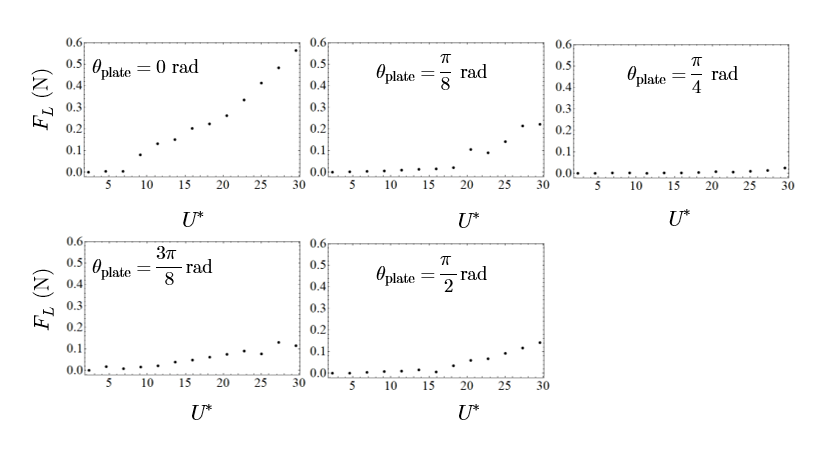
\includegraphics[width=1.0\textwidth]{liftForceRMS.png}
  \caption{Lift force variation with respect to \ured{} and \ptlt{}.}
  \label{fig:liftevo}
\end{figure}

Now we are going to see how the two dominant components of lift evolves with respect to \ured{} and \ptlt{}.

\begin{figure}[h]
  \centering
  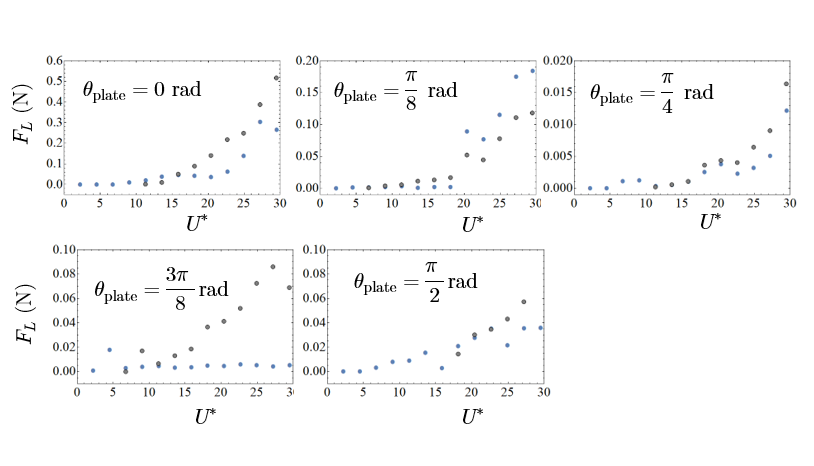
\includegraphics[width=1.0\textwidth]{liftComponentRMS.png}
  \caption{The evolution of the two most dominant components of lift after its decomposition using EEMD, against \ured{} and \ptlt{}.}
  \label{fig:liftcomp}
\end{figure}

Now let us see how the ratio between two dominant components of the lift signal evolves with respect to \ured{} and \ptlt{}.

\begin{figure}[h]
  \centering
  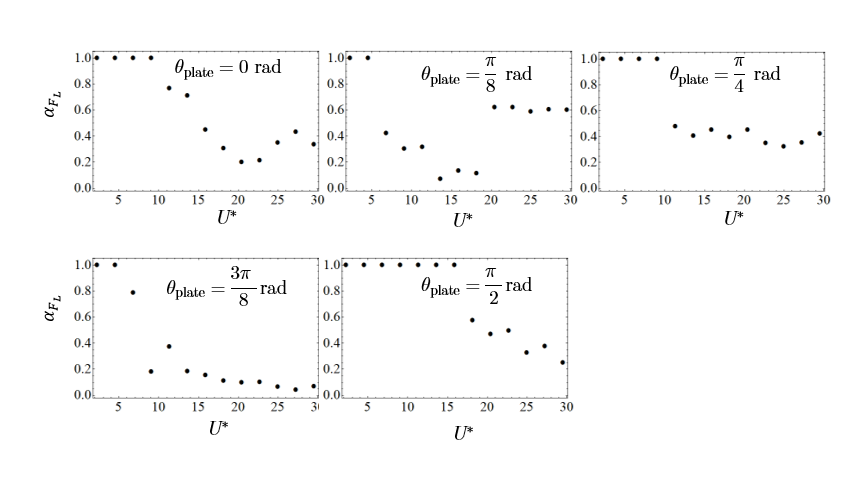
\includegraphics[width=1.0\textwidth]{liftComponentRatio.png}
  \caption{The evolution of the ratio between two dominant components of the lift signal with respect to \ured{} and \ptlt{}.}
  \label{fig:liftcomprat}
\end{figure}

\newpage

\section{Chapters completed and progress to date}

\section{Factors impeding the progress of research}

\printbibliography

\end{document}
